\documentclass[crop,tikz]{standalone}
\usetikzlibrary{backgrounds}
\colorlet{blue}{cyan}
\tikzset{
  inverted/.style = {
    every path/.style = {draw=white,text=white},
    background rectangle/.style={fill},
    show background rectangle
  }
}

\usepackage{amsmath}
\usepackage{pgfplots}

\tikzset{>=latex}
\pgfplotsset{
  compat=1.16,
  every non boxed x axis/.append style={
    axis line style={-latex}
  },
  every non boxed y axis/.append style={
    axis line style={-latex}
  }
}

\begin{document}
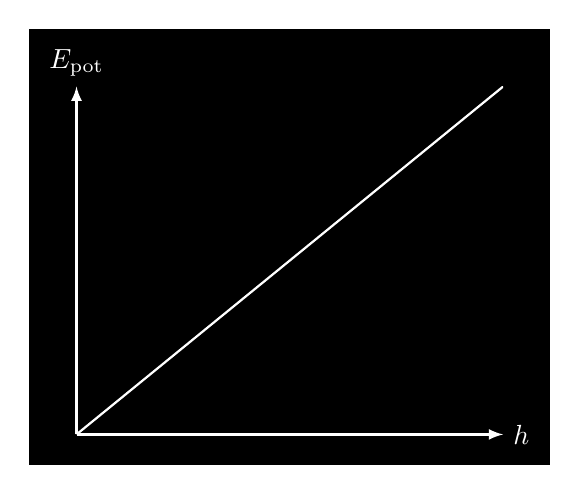
\begin{tikzpicture}[inverted,inverted]
  \begin{axis}[
    thick,
    width=7cm,
    height=6cm,
    domain=0:1,
    xmin=0, xmax={1},
    ymin={0}, ymax={1},
    samples=200,
    xlabel={$h$},
    ylabel={$E_\text{pot}$},
    axis x line=center,
    axis y line=center,
    xlabel style={right},
    ylabel style={above},
    xtick={\empty},
    xticklabels={},
    ytick={\empty},
    yticklabels={},
    ]
    \addplot[mark=none,red] {x};
  \end{axis}
\end{tikzpicture}%
\end{document}
